\documentclass{article}
\usepackage[utf8]{inputenc}
\usepackage{graphicx}
\usepackage{amsmath, amsthm, amssymb}
\usepackage{multicol}
\usepackage{svg}
\usepackage{caption}
\usepackage{vmargin}
\usepackage[hidelinks]{hyperref}

\theoremstyle{definition}
\newtheorem{defi}{Definition}[section]
\newtheorem{theorem}{Theorem}[section]
\newtheorem{proposition}{Proposition}[section]
\newtheorem{lemma}{Lemma}[section]

\title{Model Verification with Zonotopes}
\author{Xiaozhe Yao\footnote{https://yaonotes.org/lecture-notes.html}}
\date{28 Oct 2019}
\begin{document}

\maketitle
\begin{center}
    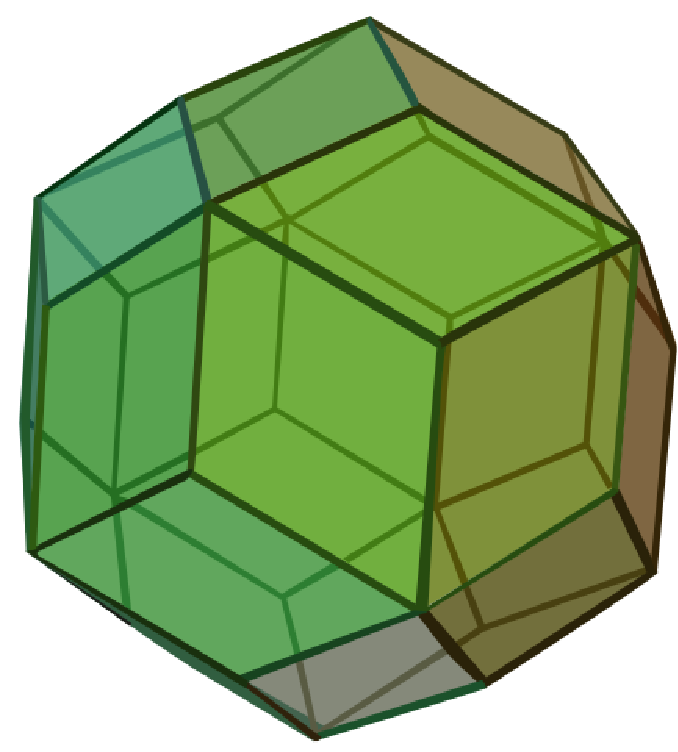
\includegraphics[width=60px]{images/zonotope.pdf}
\end{center}

\section{Introduction}

Model verification is a field of research on formally proving the output of an neural network is correct even against adversarial attacks. 

\section{Zonotopes}

\subsection{Steps}



\end{document}